\chapter{Testerbot}
\index{Testerbot|(}

Dieses Kapitel befasst sich mit dem in \xirp~vorhandenen \seegls{Testerbot} \seegls{Server}.
Dieser \seegls{Server} erzeugt f�r verschiedenste \seegls{Sensor}en Zufallswerte und sendet sie an
den verbundenen \seegls{Client}. Dadurch ist es m�glich neue Plugins zu Testen. Der
\seegls{Testerbot} kann auch dazu verwendet werden, die Anwendung zu demonstieren, ohne
dass eine aufw�ndige Roboter-Simulation oder ein echter Roboter benutzt werden m�ssen.

\newpage

\section{Kontrolloberfl�che}
\index{Testerbot!Kontrolloberfl�che}
Der \seegls{Testerbot} \seegls{Server} kann bequem aus der Anwendung heraus gestartet werden. �ber
den Men�eintrag \texttt{Extras --> Testerbot ausf�hren} wird die
Kontrolloberfl�che aufgerufen. Diese Oberfl�che ist in Abbildung
\ref{img:testerbot:control:off} auf Seite \pageref{img:testerbot:control:off} zu
sehen.

\begin{figure}[ht]
    \centering
    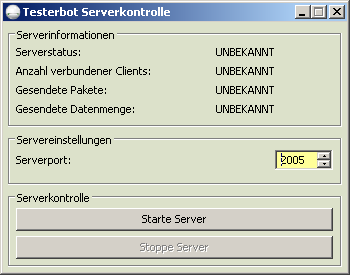
\includegraphics[width=.75\textwidth]{images/tbserverctrl}
    \caption{Die Testerbot Kontrolloberfl�che - Server abgeschaltet.}
    \label{img:testerbot:control:off}
\end{figure}

Die Kontrolloberfl�che ist in drei Bereiche aufgeteilt.

\begin{itemize}
  \item Serverinformationen
  \item Servereinstellungen
  \item Serverkontrolle
\end{itemize}

Die einzelnen Bereiche werden in den folgenden Abschnitten genauer beschrieben.
In Abbildung \ref{img:testerbot:control:on} auf Seite
\pageref{img:testerbot:control:on} ist die Oberfl�che mit aktiviertem \seegls{Server} zu
sehen.

\begin{figure}[ht]
    \centering
    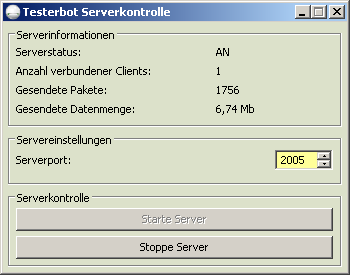
\includegraphics[width=.75\textwidth]{images/tbserverctrl_an}
    \caption{Die Testerbot Kontrolloberfl�che - Server angeschaltet.}
    \label{img:testerbot:control:on}
\end{figure}

\newpage

\subsection{Serverinformationen}
\index{Testerbot!Kontrolloberfl�che!Serverinformationen}
In diesem Bereich werden die folgenden Informationen �ber den \seegls{Server} angezeigt.

\begin{itemize}
  \item Serverstatus (An oder Aus)
  \item Anzahl verbundener Clients
  \item Gesendete Pakete
  \item Gesendete Datenmenge
\end{itemize}

\subsection{Servereinstellungen}
\index{Testerbot!Kontrolloberfl�che!Servereinstellungen}
Die einzige Einstellung die in der Oberfl�che gemacht werden kann ist die
Einstellung des Serverports. Der Standardwert ist \texttt{2005}. Ein neuer Wert
wird bei einem Neustart des \seegls{Server} benutzt.

\subsection{Serverkontrolle}
\index{Testerbot!Kontrolloberfl�che!Serverkontrolle}
In diesen Bereich gibt es zwei Kn�pfe. Nur jeweils einer ist aktiv. Die
Bezeichnung der Kn�pfe spricht f�r sich selbst und seine Funktion.

\begin{itemize}
  \item Starte Server
  \item Stoppe Server
\end{itemize}

Wird die Kontrolloberfl�che geschlossen, wird auch automatisch der \seegls{Server}
beendet. Daher muss die Oberfl�che immer angezeigt werden, wenn der \seegls{Server}
laufen soll. Die Oberfl�che kann allerdings minimiert werden.

\section{Gesendete Werte}
Der \seegls{Server} sendet Werte f�r diverse \seegls{Sensor}en. Die unterst�tzten \seegls{Sensor}en werden
im folgenden beschrieben.

\subsection{Energiequelle}
Es werden Werte f�r zwei Energiequellen gesendet.

\subsection{Infrarot}
Es werden Werte f�r vier Infrarotabstandssensoren gesendet.

\subsection{Ultraschall}
Es werden Werte f�r vier Untraschallabstandssensoren geliefert.

\subsection{Temperatur}
Es wird ein Temperaturwert gesendet.

\subsection{Thermopile}
\index{Live-Diagramm}
\index{Aufzeichungen}
Es wird ein Termopile-Array Scan geliefert. Dieser Scan besteht aus 32 mal 8
Werten. Daher ist dieser \seegls{Sensor} nicht f�r Aufzeichungen und Live-Diagramm
verwendbar.

\subsection{CO$_2$}
Es wird ein Kohlendioxidwert geliefert.

\subsection{Kompass}
Es wird ein Himmelsrichtungswert gesendet.

\subsection{Geschwindigkeit}
Es wird ein Geschwindigkeitswert gesendet.

\subsection{Neigung}
Es werden zwei Werte f�r die horizontale und vertikale Neigung geliefert.

\subsection{Laserscanner}
\index{Live-Diagramm}
\index{Aufzeichungen}
Es wird ein \seegls{Laserscanner} Scan geliefert. Dieser Scan besteht aus mehr als 600
einzelnen Werten, so dass dieser \seegls{Sensor} nicht f�r Aufzeichungen und Live-Diagramm
verwendbar ist.

\subsection{Nachrichten}
Es werden diverse Zufallstextnachrichten vom \seegls{Server} gesendet. Diese k�nnen z.B.
zum Testen der Sprachausgabe benutzt werden.

\index{Testerbot|)}
